\documentclass[tikz]{standalone}

\usepackage[latin1]{inputenc}
\usepackage{tikz}

% GNUPL
\begin{document}
\pagestyle{empty}


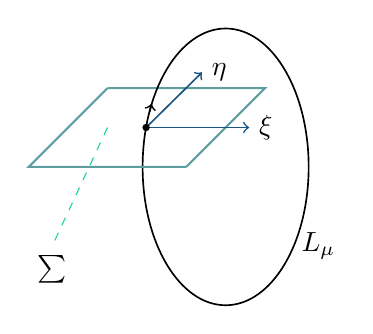
\begin{tikzpicture}
    \draw[color={rgb,255:red,95; green,158; blue,160},thick] (-1,4) -- (1,4) -- (0,3);
    \draw[semithick] (0.5,3) ellipse (30pt and 50pt);
    \draw[color={rgb,255:red,95; green,158; blue,160},thick] (0,3) --(-2,3) -- (-1,4);
    \draw[dashed,color={rgb,255:red,28; green,211; blue,162}] (-1,3.5) -- (-1.7,2);
    \coordinate [label=-90:$\sum$] (8) at (-1.7,2);
    \draw[semithick][->] (-0.465,3.7) -- (-0.44,3.8);
    \draw[semithick, color={rgb,255:red,27; green,85; blue,131}][->] (-0.51,3.5) -- (0.2,4.2);
    \draw[semithick, color={rgb,255:red,27; green,85; blue,131}][->] (-0.51,3.5) -- (0.8,3.5);
    \coordinate [label=0:$\eta$] (8) at (0.2,4.2);
    \coordinate [label=0:$\xi$] (8) at (0.8,3.5);
    \coordinate [label=0:$L_{\mu}$] (8) at (1.34,2);
    \draw[semithick][fill] (-0.51,3.5) ellipse (1pt and 1pt);

 %    \draw[semithick] [->] (0.5,8) -- (6,8) node[right] {$U_1$};
 %    \draw[semithick] [->] (0.5,8) -- (1,8);
 %    \draw[semithick] [->] (4.5,8) -- (3.5,8);
 %    \draw[semithick] [->] (4.5,8) -- (5.5,8);
 %    \draw [fill] (1.5,8) circle [radius=0.05];
 %    \draw [fill] (4.5,8) circle [radius=0.05];
 %    \draw[semithick] (3,7.9) -- (3,8.1);
 %    \coordinate [label=-90:$-\sqrt{\frac{\mu}{l}}$] (8) at (1.5,8);
 %    \coordinate [label=-90:$\sqrt{\frac{\mu}{l}}$] (8) at (5.5,8);
 %    \coordinate [label=-90:$0$] (8) at (3,8);


 %    \draw[semithick] [->] (0,3) -- (7.5,3) node[above] {$U_1$};
 %    \draw[semithick] [->] (0,3) -- (0.3,3);
 %    \draw[semithick] [->] (3.5,3) -- (3.2,3);
 %    \draw[semithick] [->] (5.8,3) -- (6,3);
	% \draw[semithick] [->] (3,1) -- (3,6) node[above] {$U_3$};
	% \draw[semithick] [->] (2,2) -- (6,6) node[above] {$U_2$};
	% \draw[teal, densely dashed][fill = teal, opacity=0.2]  (0.5,0.5) -- (2.5,2.5) -- (2.5,6.5) -- (0.5,4.5) -- (0.5,0.5);
	% \draw[teal,densely dashed][fill = teal, opacity=0.2]  (3.5,0.5) -- (5.5,2.5) -- (5.5,6.5) -- (3.5,4.5) -- (3.5,0.5);	
 %    \draw [red,thick] (1.5,3) to [out=0,in=0] (1.5,3.45) to [out=180,in=90] (1.1,3) to [out=-90,in=180] (1.5,2.35) to [out=0,in=-90] (2,3) to [out=90,in=0] (1.5,4) to [out=180,in=90] (0.7,3) to [out=-90,in=180] (1.5,1.8);
 %    \draw [red,thick] [->] (1.5,4) --(1.56,4);
	% \draw [fill] (1.5,3) circle [radius=0.05]; 
 %    \draw [red,thick] [->] (-1.05,4) --(-1,4);
 %    \draw [red,thick] (-1.2,3.8) to [out=90,in=180] (-1,4) to [out=0,in=0] (-0.8,2)to [out=180,in=180] (-0.2,3.5) to [out=0,in=90] (0.3,3) to [out=-90,in=0] (0,2.6) to [out=180,in=180] (0.2,3.2) to [out=0,in=90] (0.45,3);
 %    \draw [red,thick] (4.5,2) to [out=180,in=-90] (3.6,3) to [out=90,in=180] (4.5,3.8) to [out=0,in=90] (5,3) to [out=-90,in=0] (4.5,2.6) to [out=180,in=-90] (4.1,3) to [out=90,in=90] (4.5,3);
 %    \draw [red,thick] [->] (4.5,3.8) --(4.51,3.8);
 %    \draw [red,thick] [->] (5.9,4) --(5.91,4);
 %    \draw [fill] (4.5,3) circle [radius=0.05];
 %    \draw [red,thick] (5.7,2) to [out=180,in=180] (5.9,4) to [out=0,in=90] (6.4,3) to [out=-90,in=0] (6.2,2.5) to [out=180,in=-90] (5.9,3) to [out=90,in=180] (6.5,3.4) to [out=0,in=90] (6.9,3) to [out=-90,in=0] (6.8,2.7) to [out=180,in=-90] (6.6,3) to [out=90,in=180] (7,3.2);

	% %\mu=0
	% \coordinate [label=-90:$\mu \equiv0$] (8) at (10.5,9);

 %    \draw[semithick] [->] (8,8) -- (13,8) node[right] {$U_1$};
 %    \draw[semithick] [->] (10.5,8) -- (11,8);
 %    \coordinate [label=-90:$0$] (8) at (10.5,8);
 %    \draw [fill] (10.5,8) circle [radius=0.05];

 %    \draw[semithick] [->] (8,3) -- (13,3) node[above] {$U_1$};
 %    \draw[semithick] [->] (8,3) -- (9,3);
 %    \draw[semithick] [->] (11.5,3) -- (12,3);
 %    \draw[teal,densely dashed][fill = teal, opacity=0.2] (9.5,0.5) -- (11.5,2.5) -- (11.5,6.5) -- (9.5,4.5) -- (9.5,0.5);
 %    \draw [red,thick] (11,2) to [out=180,in=-90] (9.8,3) to [out=90,in=180] (10.5,4) to [out=0,in=90] (11,3) to [out=-90,in=0] (10.5,2.6) to [out=180,in=-90] (10.2,3) to [out=90,in=180] (10.5,3.2);
 %    \draw [red,thick] [->] (10.5,4) --(10.51,4);
 %    \draw [red,thick] (8,4.5) to [out=30,in=90] (9,3) to [out=-90,in=0] (8.5,2.3) to [out=180,in=-90] (8.2,3) to [out=90,in=180] (9.1,3.7) to [out=0,in=20] (9.25,2.8);
 %    \draw [red,thick] [->] (8.4,4.54) --(8.41,4.54);
 %    \draw [red,thick] (11.5,4.5) to [out=-30,in=0] (11.8,2.3) to [out=-180,in=180] (11.9,3.5) to [out=0,in=0] (12.5,2.5) to [out=180,in=180] (12.8,3.3);
 %    \draw [red,thick] [->] (11.7,4.35) --(11.72,4.34);
 %    \draw [fill] (10.5,3) circle [radius=0.05];

 %    %\mu>0
 %    \coordinate [label=-90:$\mu>0$] (8) at (16.5,9);

 %    \draw[semithick] [->] (14,8) -- (19,8) node[right] {$U_1$};
 %    \draw[semithick] [->] (16,8) -- (17,8);


 %    \draw[semithick] [->] (14,3) -- (19,3) node[above] {$U_1$};
 %    \draw[semithick] [->] (15,3) -- (16,3);
 %    \draw [red,thick] (14,4.5) to [out=30,in=0] (15,2) to [out=180,in=180] (16,3.8) to [out=0,in=0] (16.5,2.5) to [out=180,in=180] (17.2,3.5) to [out=0,in=0] (17.8,2.6) to [out=180,in=180] (18.4,3.2); 
 %    \draw [red,thick] [->] (14.5,4.5) --(14.51,4.495);
\end{tikzpicture}


\end{document}